\section{Методы моделирования ДНК в динуклеотидном приближении}

Описание конформации ДНК в виде набора геометрических параметров, определяющих взаимное расположение соседних нуклеотидных пар относительно друг друга, может использоваться как для исследования структуры ДНК, так и для создания физических моделей гибкости ДНК. Последние могут быть встроены в алгоритмы интегративного моделирования ДНК и ДНК-белковых комплексов. В данном разделе излагаются представления о  параметрах геометрии ДНК, эмпирических силовых полях для описания энергии изгиба ДНК в динуклеотидном приближении, а также программные продукты и методы моделирования, включая разработки научной группы автора.

\subsection{Описание геометрии ДНК}
Планарность азотистых оснований нуклеотидов и относительная планарность комплементарных пар оснований в двухцепочечной спирали ДНК позволяет применить для описания их взаимного расположения математический формализм, в котором основания или пары оснований представлены в виде плоских элементов с двумя уникальными гранями, отличимыми друг от друга из-за асимметрии оснований (см. Рис. \ref{fig:p1:DNA_param}). Разработке данных подходов способствовали работы Р. Дикерсона \cite{dickerson_definitions_1989}, В.Б. Журкина, В.И.Иванова,  В.П.Лысова \cite{zhurkin_anisotropic_1979}, В. Олсон, К. Лу \cite{lu_3dna_2003}, М. Эль Хассана, К. Калладайна \cite{el_hassan_assessment_1995} и др. Ниже сформулируем принятые на сегодняшний день подходы и алгоритмы.

Каждое азотистое основание (см. Рис. \ref{fig:p1:DNA_param}б) можно представить в виде твердого тела (при изображении обычно используются плоские прямоугольные параллелепипеды) и связанной с этим твердым телом системы отсчета. В 1999 на семинаре в Цукубе были приняты (а позднее утверждены совместной комиссией по биохимической номенклатуре Международного союза биохимии и молекулярной биологии и Международного союза теоретической и прикладной химии  (JCBN)) стандарты эталонной геометрии (расположения атомов) в идеализированных азотистых основания нуклеиновых кислот и их идеализированных Уотсон-Криковских парах \cite{olson_standard_2001}. Данные эталонной геометрии заданы в виде координат атомов относительно стандартной системы отсчета введенной для Уотсон-Криковских пар. При анализе структуры ДНК проводится совмещение эталонного основания или пары оснований с реальными по методу минимизации среднеквадратичного отклонения атомов (RMSD), таким образом каждому реальному основанию можно сопоставить, связанную с ним систему координат (см. Рис. \ref{fig:p1:DNA_param}в). В стандартной системе отсчета ось Z перпендикулярна плоскости основания и в структуре В-ДНК совпадает с направлением 5'-3' цепи ДНК для левого основания на Рис. \ref{fig:p1:DNA_param}в, ось Y параллельна линии соединяющей C1' атомы нуклеотидов, ось X направлена в сторону большой бороздки ДНК и совпадает с осью псевдосимметрии идеальной Уотсон-Криковской пары. Таким образом, в силу наличия оси псевдосимметрии эталонные координаты необходимо задать для оснований, когда они находятся в левом положении на Рис. \ref{fig:p1:DNA_param}в, координаты для их положения с правой стороны могут быть получены путем преобразования симметрии.

Определив положения систем отсчета, связанных с основаниями или парами оснований, можно ставить задачу о вычислении геометрических параметров взаимного расположения твердых тел, характеризуемыми этими системами отсчета. Из геометрии известно, что для описания взаимного расположения двух твердых тел относительно друг друга, необходимо шесть параметров, три из которых описывают поступательные степени свободы, а три вращательные. Номенклатура таких параметров была утверждена в 1988 году и носит название ``Кембриджского согласия'' (Cambridge Accord) \cite{dickerson_definitions_1989}.
Поступательные степени свободы для взаимного расположения оснований относительно друг друга носят названия Shear, Stretch, Stagger для смешения по осям X, Y, Z, соответственно (Рис. \ref{fig:p1:DNA_param}д). В случае определения этих параметров для Уотсон-Криковской пары M-N, по соглашению, систему координат основания N предварительно вращают вокруг оси X на 180 градусов. Вследствие этого, если рассматривать ту же самую пару как пару N-M, угловой параметр Buckle, обсуждаемый далее, поменяет знак на противоположный. Также при рассмотрении Уотсон-Криковской пары в обратном направлении (N-M вместо M-N) поменяет свой знак параметр Shear, но не параметры Stretch и Stagger. В случае рассмотрения Хугстиновских пар приняты другие правила, которые рассматривать здесь не будем.

Аналогично можно ввести параметры взаимного расположения пар оснований вдоль цепи ДНК, они носят название Shift, Slide, Rise для смещений вдоль осей X, Y, Z, соответственно. При рассмотрении двухцепочечной B-формы ДНК для вычисления данных параметров нам необходимо выбрать направление одной из цепей ДНК в качестве референсного, которое будет задавать направление последовательного рассмотрения пар оснований для вычисления параметров их взаимного расположения. При вычислении параметров в обратном направлении (в качестве референсной цепи задается комплиментарная цепь) знак параметра Shift поменяется на противоположный, а параметры Slide и Rise не изменят знака.

Вычисление параметров вращения оснований и пар оснований относительно друг друга представляет собой более сложную задачу, поскольку в отличие от преобразований смещения в трехмерном пространстве группа преобразований вращения являет некоммутативной, то есть зависит от последовательности применения операций вращения. Так в механике для описания вращения твердых тел зачастую используется углы Эйлера или матрицы поворота вокруг осей системы координат. Однако преобразования описываемые данными углами необходимо выполнять в определенной последовательности, конечный результат сложным образом зависит от всех трех углов. В случае описания взаимного расположения оснований ДНК таким образом углы Эйлера будут иметь трудно интерпретируемый физический смысл. Отдельной проблемой является то, что при изменении направления рассмотрения преобразований (например, M-N  вместо N-M или рассмотрении динуклеотидных переходов вдоль по одной и другой цепи ДНК) численные значения параметров вращения будут отличаться. Данная проблема была очевидна с конца 1970-ых годов (в 1981 году была установлена первая кристаллическая структура ДНК - додекамер Дрю-Дикерсона\cite{drew_structure_1981}), обсуждалась на встрече 1988 года в Кембридже (``Cambridge Accord'').  Для разрешения данной проблемы был сформулирован ряд подходов, которые для определения и вычисления параметров вращения оснований ДНК вводят понятие дополнительной системы отсчета, находящейся по середине между рассматриваемыми системами отсчета (см. напр. работу 1979 года В.Б. Журкина и др. \cite{zhurkin_anisotropic_1979}). Используя дополнительную систему отсчета можно сформулировать определение параметров вращения, которые будут независимы от направления рассмотрения преобразования.  Наиболее используемый подход был предложен Эль Хассаном и Калладайном и описан в статьях \cite{el_hassan_assessment_1995,lu_structure_1997}. Рассмотрим этот подход на примере расчета динуклеотидных параметров вращения Twist, Roll, Tilt (Рис. \ref{fig:p1:DNA_param}е), расширение данного подхода на параметры вращения оснований относительно друг друга Buckle, Propeller, Opening может быть произведено по аналогии. 

Для вычисления углов Twist, Roll и Tilt вводится система отсчета (``mid-step reference frame''), находящаяся по середине межу системами отсчета, связанными с последовательными парами оснований (см. Рис. \ref{fig:p1:DNA_param}г). Для преодоления проблемы некоммутативности операций вращения используется следующий прием. Вращение систем отчета друг относительно друга может быть представлено как вращение вокруг оси Z (Twist) на угол $\Omega$, а затем отклонение оси Z на некоторый угол $\Gamma$ вокруг какой-либо оси перпендикулярной оси Z (называемой остью RollTilt). В случае работы относительно промежуточной системы отчета (``mid-step reference frame'') процедура разлагается на поворот верхнего основания на угол $\Omega/2$ и угол $\Gamma/2$, а нижнего на угол $-\Omega/2$ и угол $-\Gamma/2$, относительно оси RollTilt, положение которой задается углом $\phi$ относительно оси Y промежуточной системы отсчета. Углы Roll ($\rho$) и Tilt ($\tau$) определяются векторным разложением по формулам:
\begin{eqnarray}
 \rho=\Gamma \cos(\phi)\\
 \tau=\Gamma \sin(\phi)
\end{eqnarray}
Позитивный Roll в А/B и W-формах ДНК соответствует открытию малой бороздки, знак параметра Tilt зависит от направления рассмотрения ДНК. Более подробное определение методов расчета параметров в современной реализации программы 3DNA может быть найдено в \cite{lu_structure_1997}.

Можно показать, что соответствующие процедуры позволяют определить схему, которая с точностью до знака дает одинаковые значения параметров при рассмотрении ДНК как в прямом, так и в обратном направлениях.
Важной особенностью данного подхода является то, что структура ДНК может быть однозначно восстановлена по наборам рассчитанных параметров. Таким образом, можно проводить конвертацию атомистических структур в пространство параметров оснований ДНК и обратно, а также генерировать структуры с измененной последовательностью, но идентичной геометрией. 


\begin{figure}[H] 
  \center
  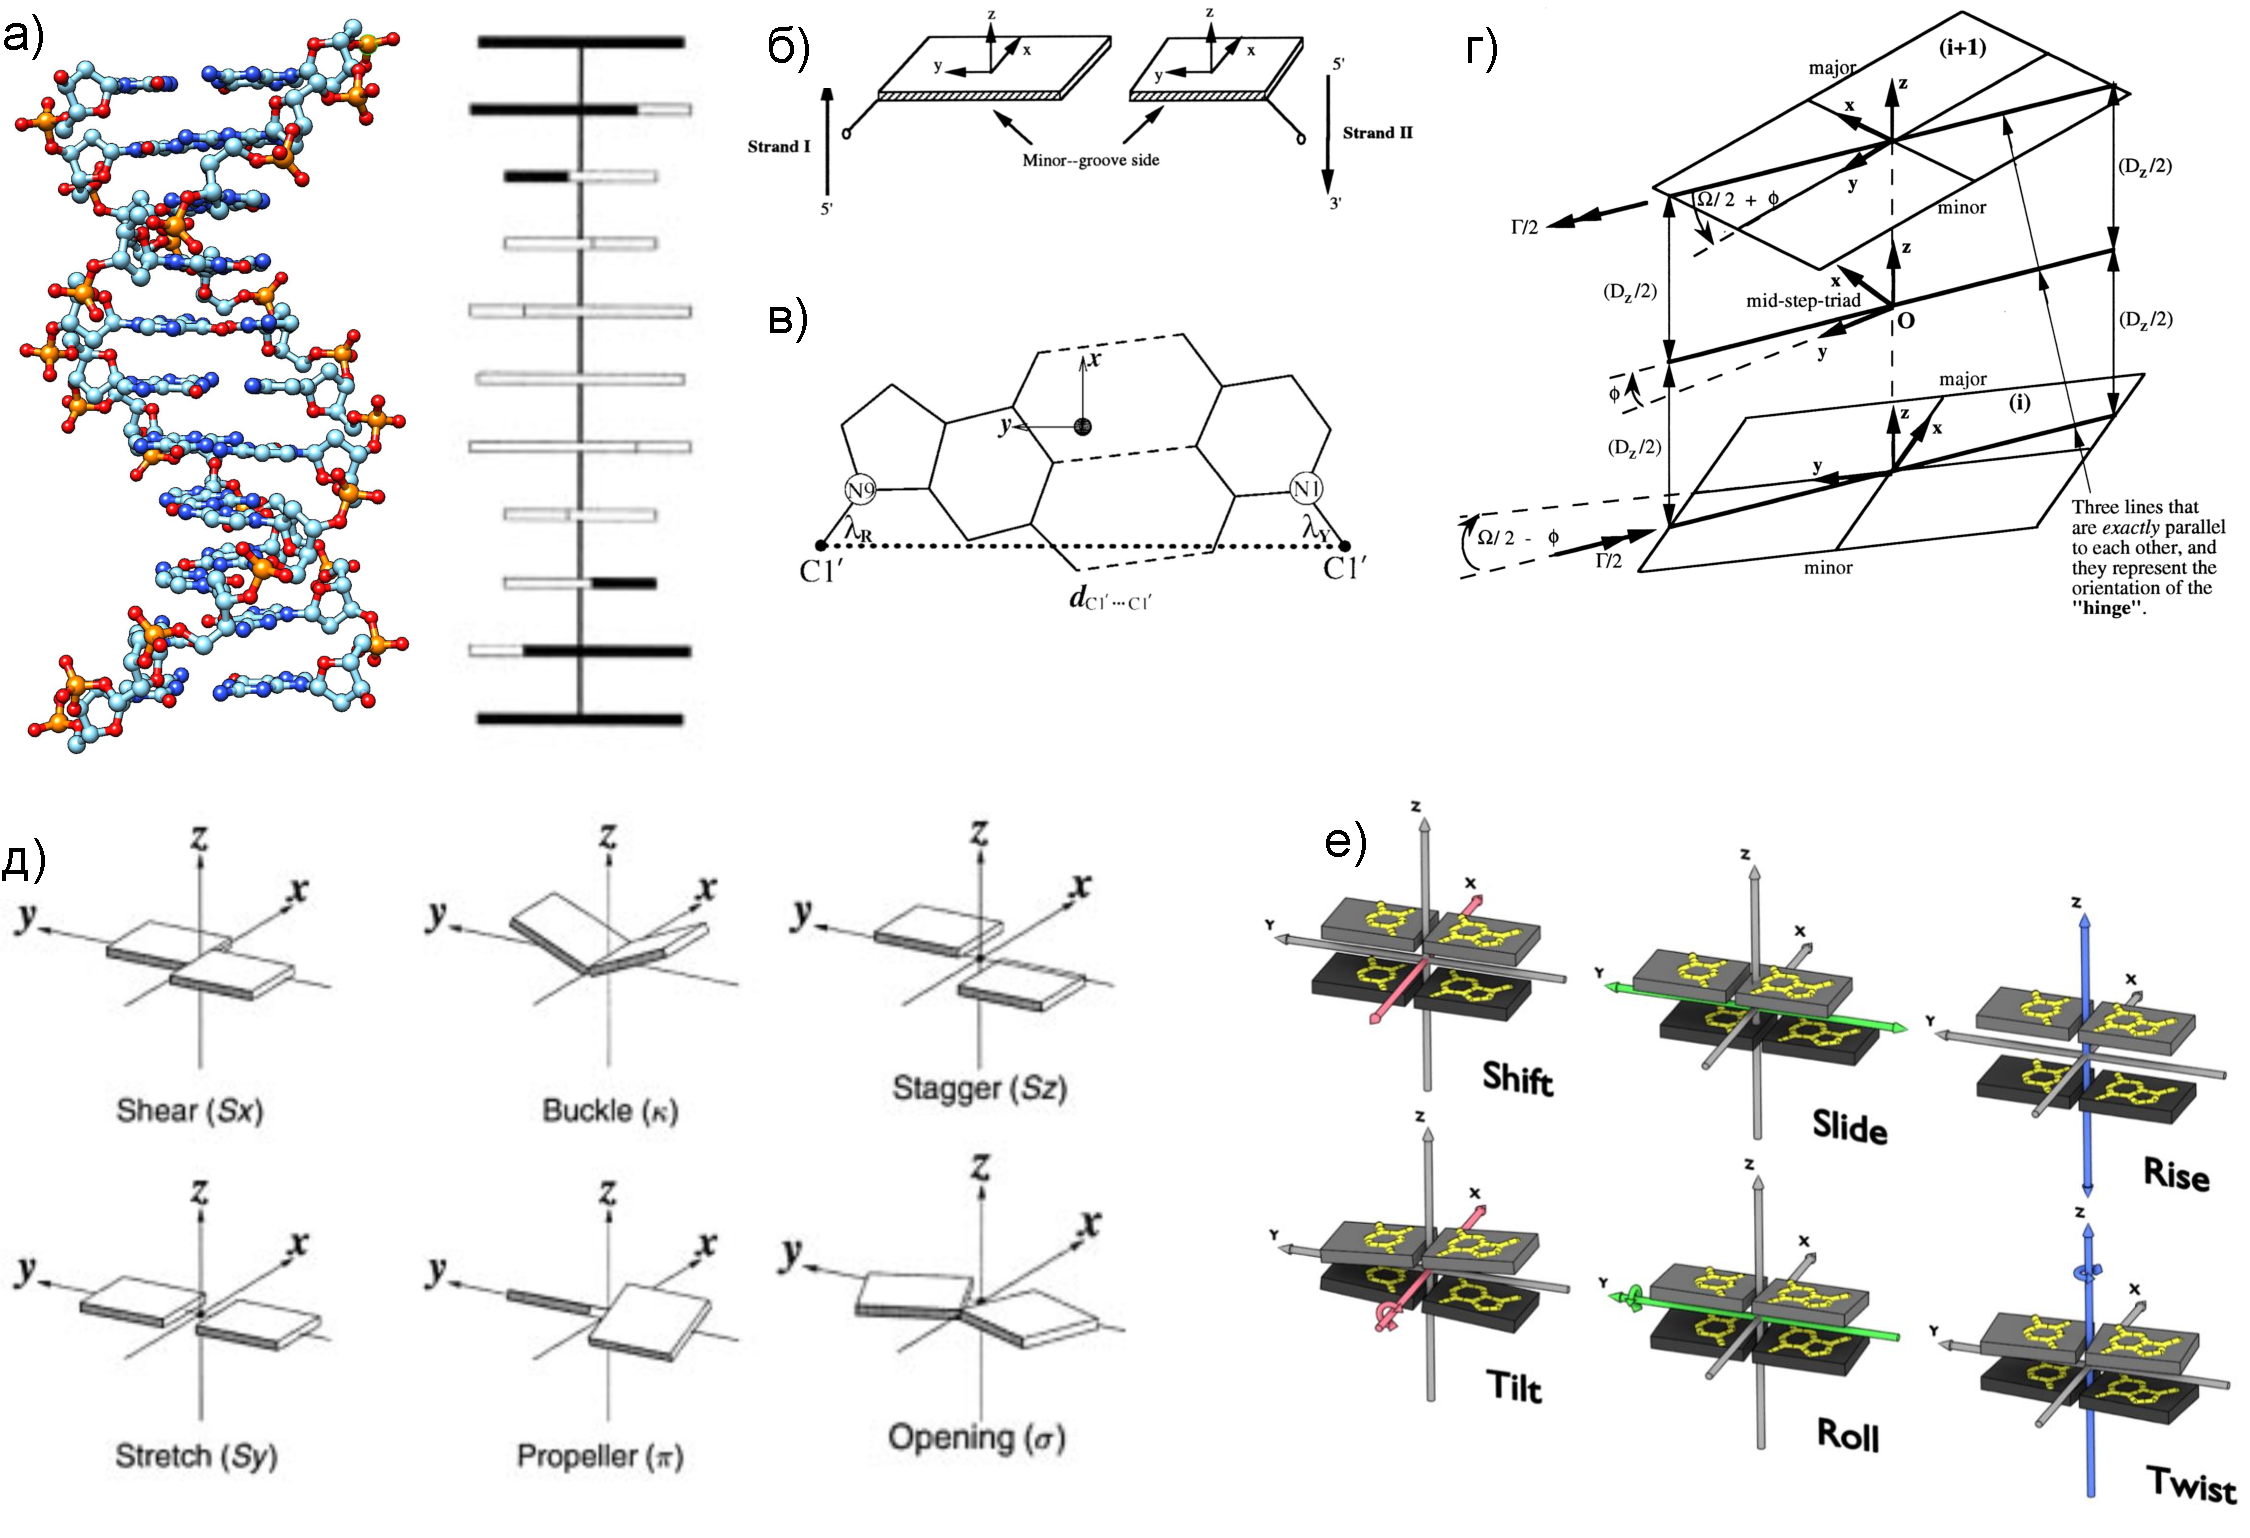
\includegraphics [width=\textwidth] {images/p1/DNA_param}
  \caption[Описание геометрии ДНК в виде геометрических параметров]{Описание геометрии ДНК в виде геометрических параметров. a) Атомистическое представление B-формы ДНК и представление в виде диаграммы по принципам Калладайна и Дрю \cite{calladine_understanding_2004}; б) представление пары оснований в виде параллелепипедов и связанные с ними системы координат \cite{el_hassan_assessment_1995}, в) система координат и ее расположение относительно пары оснований \cite{olson_standard_2001}, г) иллюстрация введения промежуточной системы отсчета между парами оснований для расчета параметров вращения  \cite{el_hassan_assessment_1995}, д) параметры взаимного расположения оснований в паре оснований \cite{lu_3dna_2003}, е) параметры взаимного расположения пар оснований относительно друг друга вдоль ДНК.} 
  \label{fig:p1:DNA_param}
\end{figure}

\subsection{Эмпирические константы жесткости изгиба ДНК}
Возможность задания общей конформации ДНК в виде набора 12 параметров, определяющих взаимное расположение азотистых оснований, позволяет поставить вопрос о возможности задания некоторого силового поля, способного описывать энергию различных конформаций двухцепочечной ДНК как функцию этих параметров. Для двухцепочечной ДНК любой последовательности, содержащей N пар оснований, 6(N-1) параметров будут описывать взаимное расположение пар оснований относительно друг друга. Формально с точки зрения статистической физики, поскольку каждой конкретной конформации ДНК однозначно можно сопоставить численные значения этих параметров и параметры являются независимыми, то набор этих параметров можно рассматривать как набор обобщенных координат (координат реакции), в пространстве которых может быть задана функция свободной энергии.

В общем случае данная функция будет иметь сложную структуру. Для того, чтобы такой формализм мог быть использован на практике, необходимо вводить ряд приближений относительно структуры данной функции. Наиболее используемым является, так называемое, динуклеотидное аддитивное приближение. Предполагается, что функция свободной энергии аддитивно складывается из компонент, описывающих вклады отдельных динуклеотидных шагов:

\begin{equation}
    F_{tot}(\{\theta^1_j\}, \{\theta^2_j\}, ... , \{\theta^{N-1}_j\})=\sum_{i=1}^{N-1}F_k(\{\theta^k_j\})
\end{equation}
где $k$ - номер динуклеотидного шага, $\{\theta^k_j\}$ - набор 6 переменных Roll, Tilt, Twist, Shift, Slide, Stagger для динуклеотидного шага $k$. 

Следующим упрощением является введение гармонического приближения для представления свободной энергии каждого динуклеотидного шага в виде разложения функции до второго порядка вблизи точки равновесия.
\begin{equation}
    F_k(\{\theta^k_j\})=F_0+\frac{1}{2}\sum_{i=1}^{6}\sum_{j=1}^{6}f_{ij}\Delta\theta^k_{i}\Delta\theta^k_{j}\\
    \Delta\theta^k_{i}=(\theta^k_{i}-\hat{\theta}^k_{i})
    \label{DNA_ener}
\end{equation}
Наконец, последним важным приближением является предположение о том, что коэффициенты $f_{ij}$ и равновесные значения $\hat{\theta}^k_{i}$ зависят только от типа конкретного динуклеотидного шага и не зависят от типа соседних нуклеотидов. Такое приближение называется приближением ближайших соседей (nearest neighbor). Следует отметить, что это лишь приближение, и в некоторых  особых случаях учета ближайших соседей не хватает для адекватного описания - например, когда важны коллективные эффекты вдоль по цепи, связанные с бифуркациями водородных связей, образованием цепочек воды в малой бороздке и т.д. Например, такие эффекты известны при рассмотрении протяженных участков аденина или тимина (А-траки), которые обладают высокой изгибной жесткостью.

Оценка констант $f_{ij}$ для каждого типа динуклеотидных шагов (всего их 10: CG,CA,TA,AG,GG,AA,GA,AT,AC,GC; в силу симметрии ДНК, напр. динуклеотидные шаги AA и TT обозначают один и тот же шаг, но по разным цепям) является нетривиальной задачей. На сегодняшний день существует два подхода - анализ кристаллических структур или расчеты методами молекулярного моделирования на основе атомистических силовых полей.

Первый подход был в значительной степени реализован в работе \cite{olson_dna_1998}. Авторами был проанализирован набор из 92 комплексов белок-ДНК и построены распределения динуклеотидных параметров в этих структурах (см. Рис. \ref{fig:p1:olson_DNA_param}). Предполагается, что изучая ансамбли распределений динуклеотидных параметров в комплексах ДНК-белок, можно получить информацию о подвижности и гибкости ДНК самой по себе. Аргументация данного предположения авторами сводится к следующему. Различные белки при связывании оказывают различные воздействия на  конформацию молекулы ДНК, таким образом, при достаточно большом усреднении и рассмотрении конформации ДНК вблизи равновесия в статистике будет проявляться лишь естественная склонность ДНК к деформациям.
Более строгим образом такое предположение обосновать сложно. Однако из анализа структур белков, известно, что распределение различных параметров полипептидной цепи в глобулярных белках обладает квази-больцмановской статистикой по отношению к энергетическим функциям, описывающим их локальные взаимодействия. Например, встречаемость различных ротамеров боковых цепей аминокислот согласуется с больцмановским распределением, описываемым функцией потенциальной энергии вращения вокруг соответствующей связи. Аналогичные наблюдения имеются для экспонированности боковых цепей аминокислот в воду и энергии их гидратации \cite{shaytan_solvent_2009}. Теоретическое объяснение этого явления было дано Финкельштейном и др. \cite{finkelstein_why_1995}. Описывая белок как гетерополимер согласно модели случайных энергий (Random Energy Model), можно показать, что количество аминокислотных последовательностей, которое стабилизируют тот или иной элемент белкового фолда, экспоненциально убывает с увеличением энергии этого элемента. Таким образом, квази-Больцмановская статистика является следствием устройства энергетического спектра нативных белков, у которых должна быть одна выраженная нативная конформация, энергетический уровень которой является самым низким по энергии и отделен энергетической щелью. Следуя этой логике, можно предположить, что количество различных белков, которые могут изгибать ДНК с той или иной силой, также будет экспоненциально зависеть от энергии изгиба ДНК.
\begin{figure}[H] 
  \center
  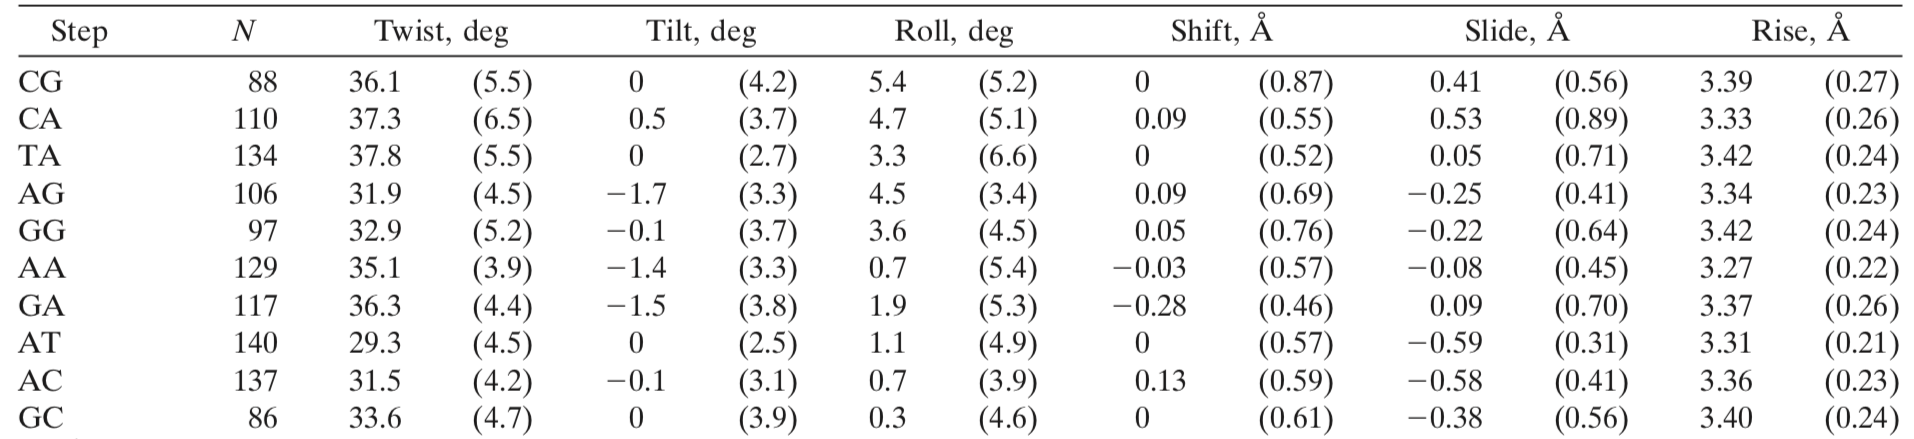
\includegraphics [width=\textwidth] {images/p1/olson_DNA_param}
  \caption{Матрица средних значений и отклонений динуклеотидных параметров из статьи \cite{olson_dna_1998}.} 
  \label{fig:p1:olson_DNA_param}
\end{figure}

Вычислив параметры отклонения ДНК в зависимости от типа динуклеотидного шага, а также дисперсии этих параметров, можно ставить задачу об оценке констант жесткости изгиба ДНК по этим различными параметрам $f_{ij}$ методом обратного гармонического анализа. В случае одномерной пружины, энергия которой описывается гармоническим законом $E=\frac{1}{2}fx^2$, распределение координаты согласно закону Больцмана будет выглядеть как $P(x) \sim \exp{-\frac{fx^2}{2kT}}$. Последнее является нормальным распределением с параметром дисперсии $\langle x^2 \rangle=kT/f$. Таким образом, мы установили связь дисперсии величины с константой жесткости.
В общем случае, когда энергия описывается функцией вида \ref{DNA_ener},  распределение состояний описывается многомерным нормальным распределением вида:
\begin{equation}
    P_{\mathbf X}(x_1,\ldots,x_k) = \frac{\exp\left(-\frac 1 2 ({\mathbf x}-{\boldsymbol\mu})^\mathrm{T}{\boldsymbol\Sigma}^{-1}({\mathbf x}-{\boldsymbol\mu})\right)}{\sqrt{(2\pi)^k|\boldsymbol\Sigma|}}
\end{equation}
где $|\boldsymbol\Sigma|=\det \boldsymbol\Sigma$, а $\boldsymbol\Sigma|$ - является матрицей ковариаций. Таким образом, несложно увидеть, что 
\begin{equation}
    \langle   \Delta\theta_{i} \Delta\theta_{j}\rangle=kT[{\boldsymbol F^{-1}}]_{ij}
\end{equation}
где ${\boldsymbol F}$ матрица коэффициентов $f_{ij}$, k - коэффициент Больцмана, $T$- конформационная температура, которую можно определить, например, сравнив получаемую гибкость с известными данными о персистентной длине. Константы жесткости доступны по адресу \url{https://web.archive.org/web/20151025043044/http://rutchem.rutgers.edu/~olson/pdna.html}.


Альтернативным подходом является вычисление характеристик динуклеотидных параметров путем молекулярного моделирования на основе атомистических силовых полей. Наиболее актуальной и современной здесь является работа \cite{walther_multi-modal_2020}. Авторы использовали наработки ABC консорциума, участники которого промоделировали методом атомистической молекулярной динамики все возможные последовательности тетрануклеотидов (всего их 136) \cite{dans_static_2019}. Из данных траекторий можно получить данные о флуктуациях различных параметров. Было показано, что распределения динуклеотидных параметров в некоторых случаях являются мультимодальными и их сложно аппроксимировать в виде одного многомерного гауссова распределения. Поэтому в данной статье некоторые распределения параметров описываются линейной комбинацией многомерных гауссовых распределений. Кроме того авторы делают попытку сделать коэффициенты $f_{ij}$ зависимыми от соседних с динуклеотидным шагом пар оснований - эффективно учитывая параметры изгибной жесткости ДНК на тетрануклеотидном уровне.

Суммируя вышесказанное, отметим достоинства и недостатки различных подходов. Гармоническое приближение при описании гибкости ДНК безусловно имеет свои ограничения, особенно в случаях, когда белок сильно деформирует ДНК. Например, в нуклеосомах динуклеотиды  пиримидин-пурин (YR) обычно выгибаются в сторону малой бороздки (параметр Roll отрицательный), в то же время из Рис. \ref{fig:p1:olson_DNA_param} видно, что в среднем в структурах динуклеотиды имеют положительный Roll, причем, динуклеотид TA (YR) больше склонен к положительному Roll, чем AT (RY). Однако предполагается, что при сильных изгибах (изломах, kinks) поверхность энергии устроена более сложным образом, и при комбинации с положительными значениями Slide - как раз AT выгоднее гнуться в сторону малой бороздки, чем TA \cite{wang_sequence-dependent_2010}. В этом плане мультимодальное приближение изгибной жесткости ДНК может являться более точным. Однако, для мультимодального приближения требуется большое количество качественных данных о динамике ДНК, которые, казалось бы, можно взять из молекулярно-динамических расчетов. Однако, здесь есть свой подводный камень - атомистические силовые поля, существующие на сегодняшний день, не совсем корректно описывают зависимость изгибной жесткости ДНК от последовательности в сравнении со структурными данными. Так, например, по данным вычислений молекулярной динамики максимальным значением параметра Roll Roll обладает динуклеотид TG \cite{pasi_muabc_2014}, а по данным анализа кристаллических структур CG.

\subsection{Программные продукты}
Для анализа геометрии ДНК был создан достаточно большое набор программных продуктов и методов, к ним можно отнести программы CompDNA\cite{gorin_b-dna_1995}, SCHNAaP \cite{lu_structure_1997}, Curves+ \cite{lavery_conformational_2009}, 3DNA \cite{lu_3dna_2008}. На данный момент наиболее используемой и поддерживаемой является программа 3DNA, которая позволяет не только анализировать структуру, но и реконструировать атомистическую структуру по набору параметров. Для анализа ширин и глубин бороздок ДНК может использовать программа Curves+.
Моделирование конформации ДНК в динуклеотидном приближении сводится к реализации либо алгоритмов минимизации конформации ДНК в пространстве параметров, либо к динамическим расчетам с помощью метода Монте-Карло. Многие такие программы разрабатывались для решения конкретных научных задач внутри научных групп, например, DNAminiCarlo (N.B. Ulyanov,
A.A. Gorin, V.B. Zhurkin), аналогичные подходы описаны в ряде статей \cite{norouzi_topological_2015,kulaeva_internucleosomal_2012}, недавно появилась программа MC-enNN и веб-сервер к ней \cite{walther_multi-modal_2020}. В нашей научной группе проводится разработка программы с открытым программным кодом PyNAMod
 \url{http://github.com/intbio/PyNAMod}, способной моделировать ДНК, включая ДНК-белковые комплексы в динуклеотидном приближении методами минимизации геометрии ДНК, а также методом цепей Монте-Карло.

\subsection{Алгоритмы интегративного моделирования}
\label{sec:p1:int_algo}
Введение дополнительных ограничений при моделировании ДНК в динуклеотидном приближении, а также учет стерических ограничений путем конвертации структуры из пространства динуклеотидных параметров в атомистическую структуру, позволяют сформулировать подходы для интегративного моделирования ДНК и комплексов-ДНК белок на основе различных экспериментальных данных.

В реализованных нами подходах при минимизации конформации ДНК в динуклеотидном приближении в энергию системы вводились дополнительные члены, соответствующее отклонению набора расстояний от целевых значений, измеренных при помощи экспериментальных методов, например, spFRET. Алгоритм действия программы изображен на Рис. \ref{fig:p1:int_mod_dinuc}. На вход программа получает начальные структуры в формате PDB. Измерения методом spFRET дают информацию о расстояниях между парами меток. Алгоритм последовательно оптимизирует координаты нуклеотидных пар таким образом, чтобы привести их геометрию в соответствие с результатами spFRET. В ходе работы алгоритма учитываются ограничения, связанные с жесткостью ДНК.


\begin{figure}[H] 
  \center
  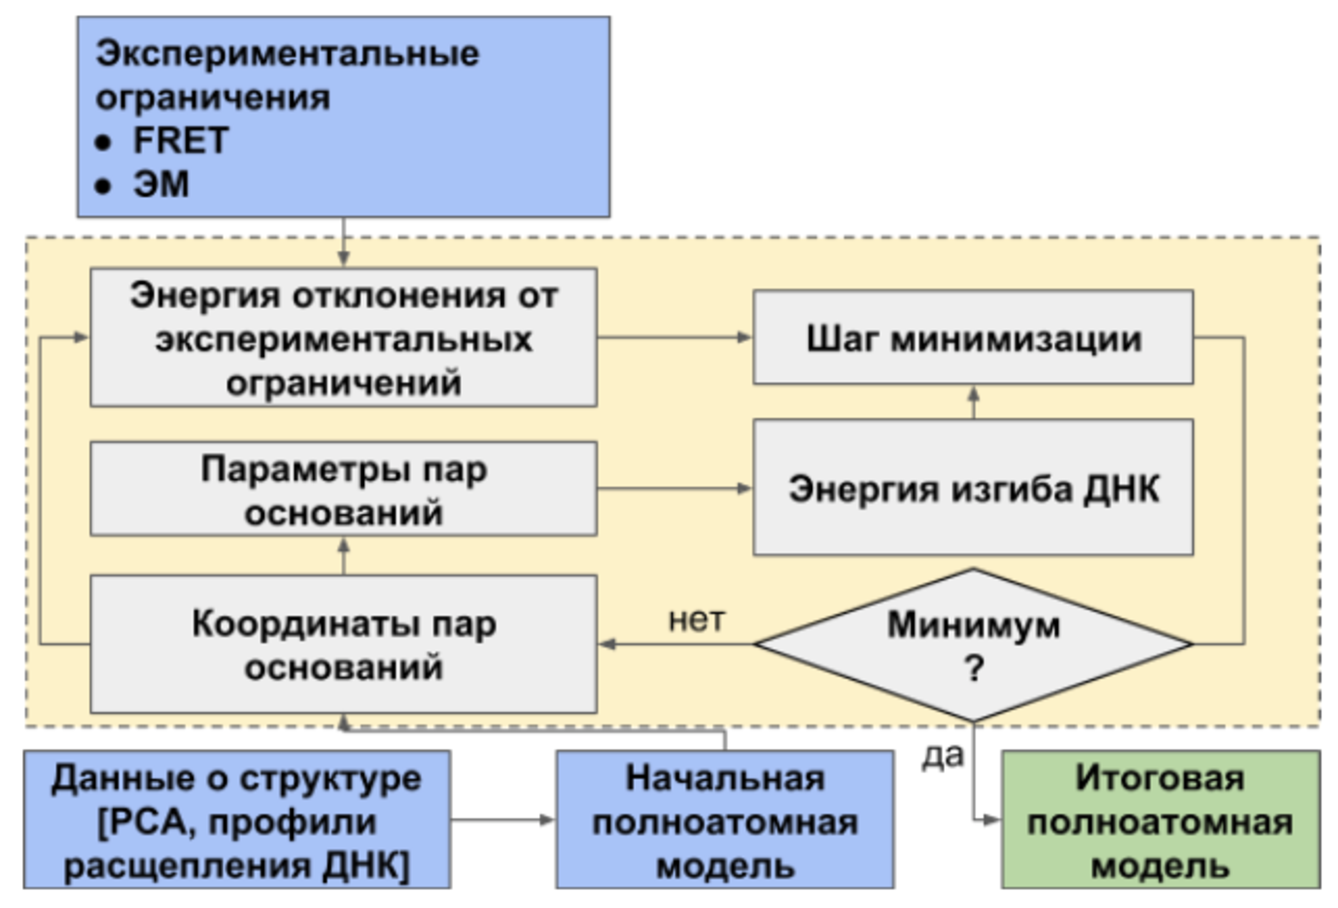
\includegraphics [width=\textwidth] {images/p1/int_mod_dinuc}
  \caption{Алгоритм интегративного моделирования на основе моделей ДНК в динуклеотидном приближении.} 
  \label{fig:p1:int_mod_dinuc}
\end{figure}